% !TEX root = ../main.tex
% Visualisierung

% Kapitel \ref{chap:daten} gibt einen "Uberblick "uber gr"o"se und Struktur der genutzten Datens"atze um nachvollziehen zu k"onnen welche Daten visualisiert werden.
In diesem Kapitel wird auf die gewählte Darstellung von Kategorien eingegangen und welche Interaktionsmöglichkeiten die Visualisierung bietet.
Darüber hinaus wird verdeutlicht, welche nicht sichtbaren Veränderungen während der Laufzeit des Programms an den Daten vorgenommen werden.
In diesem Kapitel werden die beschriebenen Datensätze aus dem Kapitel \ref{chap:daten} näher erläutert und mit ihrer visuellen Repräsentation verknüpft.

Im Gegensatz zur Visualisierung aus dem Projekt \emph{Visual Text Analytics} stehen die Verbindungen zwischen den Kategorien im Mittelpunkt der angestrebten Darstellung.
Der Ansatz aus dem vorangegangenen Projekt, möglichst viele Artikel mit ihren Ähnlichkeiten abzubilden, führt zu einer unüberschaubaren Menge an Vergleichen, die wiederum in einer Undurchsichtigkeit der dargestellten Elemente resultiert (\emph{visual clutter}).
In der vorliegenden Arbeit wird deshalb ein neuer Ansatz verfolgt, welcher sich auf die Kategorien fokussiert.
Mittels der Kategorien soll ein abstrakterer Zugang zu den Artikeln geschaffen, die Übersichtlichkeit gestärkt und die Auswahl an Artikeln auf ein Themengebiet beschränkt werden.

%  Vorhaben, eine geeignete Darstellungsform der Kategorienstruktur zu finden, folgend wird diese Struktur analysiert.
% % Die Voraussetzung dafür ist die Analyse der Kategorienstruktur der Wikipedia 
Der Grundgedanke der Arbeit liegt in der Annahme, die Kategorienstruktur als eine Hierarchie von Abstraktionsebenen zu interpretieren.
Diese Annahme wird durch eine Analyse der Kategorienstruktur überprüft.
Auf der Wikipedia-Seite \emph{Main Topic Classifications}\footnote{\url{https://en.wikipedia.org/wiki/Category:Main_topic_classifications}} wird darauf hingewiesen, dass die Kategorienstruktur nicht als strikt hierarchisch zu verstehen ist.
Daraus lässt sich schließen, dass die Kategorien in einem Graphen miteinander verbunden sein können.
Die genauere Betrachtung der Beziehungen zwischen den Kategorien verdeutlicht ihre Eigenschaften.
Besteht eine Verbindung zwischen zwei Kategorien, werden diese jeweils in der anderen Kategorie als Unterkategorie oder als Oberkategorie eingetragen. 
Daraus lässt sich folgern, dass der Graph, bestehend aus Verbindungen zwischen den Kategorien, ein gerichteter Graph ist und somit einer gewissen Ordnung folgt.

Im Folgenden wird an einem konkreten Beispiel ein Pfad von Unterkategorien exemplarisch erkundet.
Die Analyse der Wikipedia-Seite der Kategorie \emph{Computer science} und ihrer Unterkategorien zeigt, dass die Kategorien, die näher zum gewählten Stammverzeichnis \emph{Computer science} liegen, Themengebiete eher umfassend beschreiben.
Die Kategorien, die weiter vom Stammverzeichnis entfernt sind, umschreiben einen Gegenstand hingegen spezifischer.
Auf Grund dieser Beobachtungen kann davon ausgegangen werden, dass die Kategorienstruktur einer thematischen Ordnung bzw. einer thematischen Hierarchie folgt.
Am Beispiel eines Pfades der Unterkategorien des Stammverzeichnisses \emph{Computer Science} werden diese Abstraktionsebenen exemplarisch in der Abbildung~\ref{fig:cs-tree} dargestellt.

\begin{figure}
    \centering
    \begin{tikzpicture}
    \matrix (m) [matrix of nodes, column sep=4mm]
    {
        CS  & CS history                & Algorithms \& Datastructures          & Algorithms            &   \\
            & CS by year                & Artificial inteligence               &  Abstract Datatypes   & Arrays  \\
            & CS by country             & Computer architecture                 &  ...                  & Trees  \\
            & ...                       & ...                                   & Datastructures        & ...  \\
            & CS area                   & Computer security                     &                       & Queue  \\
    };
    \draw (m-1-1) -- (m-1-2);
    \draw (m-1-1) -- (m-2-2);
    \draw (m-1-1) -- (m-3-2);
    \draw (m-1-1) -- (m-5-2);
    
    \draw (m-5-2) -- (m-1-3);
    \draw (m-5-2) -- (m-2-3);
    \draw (m-5-2) -- (m-3-3);
    \draw (m-5-2) -- (m-5-3);
    
    \draw (m-1-3) -- (m-1-4);
    \draw (m-1-3) -- (m-2-4);
    \draw (m-1-3) -- (m-4-4);
    
    \draw (m-4-4) -- (m-2-5);
    \draw (m-4-4) -- (m-3-5);
    \draw (m-4-4) -- (m-5-5);
    

    \end{tikzpicture}
    \caption{Ausschnitt der Kategorienstruktur ausgehend von der Kategorienseite \emph{Computer science}}
    \label{fig:cs-tree}
\end{figure}

Zusammenfassend lässt sich aus den vorangegangenen Beobachtungen Folgendes schließen: Die Kategorien folgen untereinander einer Ordnung, welche durch die gerichteten Verbindungen zwischen den Kategorien abgebildet werden.
Diese Feststellung bildet die Basis, um aus dem gerichteten Graphen einen Baum zu konstruieren, der die Hierarchie der Kategorien abbildet.\\
Weiterhin besteht die Schwierigkeit darin, die Entstehung der Schleifen im Kategorienbaum zu verhindern und somit zu entscheiden, welche Kanten aus dem gerichteten Kategoriengraphen in den Kategorienbaum übernommen werden.
Die Konstruktion eines Baumes, der die Hierarchie abbilden soll, stellt somit kein triviales Problem dar.

Die in dieser Arbeit angewandte Methode traversiert den gerichteten Kategoriengraphen mit einer iterativen Tiefensuche, auf die im Kapitel \ref{chap:Implementierung} näher eingegangen wird, ausgehend von einer gewählten Startkategorie.
Dabei werden nur die Knoten aus dem Graphen dem Baumdiagramm hinzugefügt, die nicht bereits in diesem abgebildet sind.
Die Knoten einer Ebene werden mit dem Knoten verbunden, von dem aus eine Kante auf sie gerichtet ist.
Auf diese Art soll gewährleistet werden, dass keine Schleifen während der Konstruktion des Baumes entstehen.
In dem Kapitel~\nameref{chap:Implementierung} wird auf den verwendeten Algorithmus, welcher aus dem gerichteten Graphen ein Baumdiagramm konstruiert, näher eingegangen.

Der erste Ansatz versucht einen Kategorienbaum für \emph{sämtliche} Wikipedia-Kategorien zu erstellen.
Für einen vollständigen Kategorienbaum wird ein Stammverzeichnis gesucht, das zwei Eigenschaften erfüllt: Erstens sollen in den Unterkategorien, ausgehend vom Stammverzeichnis, ausschließlich Kategorienseiten oder Artikelseiten eingetragen sein und zweitens soll ein Stammverzeichnis so gewählt werden, dass möglichst viele Themengebiete direkt oder in Unterkategorien enthalten sind.
Die Wikipedia markiert die Kategorie \emph{Contents}\footnote{\url{https://en.wikipedia.org/wiki/Category:Contents}} als Stammverzeichnis aller Kategorienseiten.
Diese Seite ist gleichwohl ungeeignet für die Nutzung als Stammverzeichnis, da in ihr auch Kategorien aus Namensräumen außerhalb der Artikelseiten eingetragen sind.

In dieser Arbeit wird die Kategorie \emph{Main Topic Classifications} als globales Stammverzeichnis für alle Kategorien gewählt, da sie all diese Eigenschaften erfüllt.
In ihren Unterkategorien sind hauptsächlich Artikelseiten eingetragen. 
Die direkten Unterkategorien enthalten 22 unterschiedliche Themengebiete, die den Inhalt der Wikipedia abbilden.

Sucht ein Nutzer nach einer Kategorie, ist es folglich möglich, ihm, ausgehend von der gesuchten Kategorie, einen Ausschnitt des vollständigen Kategorienbaums zu zeigen.
Das Problem der dargestellten Hierarchie ist, dass bestimmte Verbindungen der gesuchten Kategorie oder ihren Unterkategorien nicht dargestellt werden, weil sie bereits in einem höheren Pfad des vollständigen Kategorienbaums abgebildet sind.
In der Abbildung~\ref{fig:two-trees} wird dieses Phänomen verdeutlicht.

\begin{figure}
    \centering
    \begin{tikzpicture}
        \matrix (m) [matrix of nodes, column sep=4mm, right delimiter=\}] at (0,5)
            {
                CS  &|[red]|CS by year        &|[red]| 20th in CS                    \\
                    & CS area           &|[red]| 21th in CS                    \\
                    & CS by country     & \\
                    &                   & \\
                    &                   & History of computer companies \\
                    & ...               & ...                           \\
                    & CS history        & History of software           \\
            };
            \draw (m-1-1) -- (m-1-2);
            \draw (m-1-1) -- (m-2-2);
            \draw (m-1-1) -- (m-3-2);
            \draw (m-1-1) -- (m-7-2);
            
            \draw (m-1-2) -- (m-1-3);
            \draw (m-1-2) -- (m-2-3);
            \draw (m-7-2) -- (m-5-3);
            \draw (m-7-2) -- (m-6-3);
            \draw (m-7-2) -- (m-7-3);
            
            % \draw[thick, blue ] (-4,5) rectangle (5.2,3);
            \node (a) at (6.5,5) {(a)};
            \node (b) at (6.5,0) {(b)};

        \matrix (l) [matrix of nodes, column sep=4mm, right delimiter=\}] at (0,0)
            {
                & CS history  & History of computer companies                    \\
                &             & ...                 &        \\
                &             & |[red]|CS by year          & \\
                &             & |[red]|20th in CS          & \\
                &             & |[red]|21th in CS          &  \\
                &             & ...                 &   \\
                &             & History of software &          \\
            };
            \draw (l-1-2) -- (l-1-3);
            \draw (l-1-2) -- (l-3-3);
            \draw (l-1-2) -- (l-4-3);
            \draw (l-1-2) -- (l-5-3);
            \draw (l-1-2) -- (l-7-3);



    \end{tikzpicture}
    \caption{Es werden zwei Kategorienbäume dargestellt, die mit den unterschiedlichen Anstäzen aus \ref{chap:visualization} konstruiert wurde. Rot markierte Kategorien aus Abbildung (b) sind in Abbildung (a) nicht unter der Kategorie \emph{CS History eingetragen}, stattdessen sind die markierten Kategotrien in anderen Pfanden des Kategorienbaums}
    \label{fig:two-trees}
\end{figure}

Der zweite Ansatz probiert, diese Ungenauigkeit in der Darstellung der Hierarchie aus dem gerichteten Graphen zu mindern.
Sucht der Nutzer nach einer Kategorie, wird, wie bereits am Anfang des Kapitels beschrieben, mit der iterativen Tiefensuche und den festgelegten Bedingungen ein neuer Kategorienbaum konstruiert.
% Dieser unterscheidet sich vom Ausschnitt des vollständigen Kategorienbaums aus dem ersten Ansatz, wie in der Abbildung~\ref{fig:two-trees} veranschaulicht wird.
Da in diesem Fall der Kategoriengraph ausgehend von der gewählten Wurzelkategorie traversiert wird, werden mehr Unterkategorien in der Hierarchie abgebildet als zuvor in dem Ansatz des vollständigen Kategorienbaums.
Dieser Kategorienbaum schafft ein genaueres Abbild der Hierarchie für die gewählte Wurzelkategorie.
Dabei ist zu beachten, dass die dargestellte Hierarchie immer nur eine Interpretation des gerichteten Graphen bedeutet.

In beiden Fällen wird jedoch mit der Hierarchie der Kategorien eine \emph{Top-Down}-Struktur\footnote{\url{https://de.wikipedia.org/wiki/Top-down_und_Bottom-up}} modelliert, die genutzt werden kann, um Themengebiete zu erkunden.
Der Abschnitt~\ref{subchap: filter-vis} erklärt, wie die \emph{Top-Down}-Exploration genutzt wird, um auf Artikel zuzugreifen.
Dieser Ansatz spielt eine grundlegende Rolle in der Selektion der Artikel.
In den folgenden Abschnitten wird auf die visuelle Umsetzung und die Interaktion eingegangen.

\begin{figure}[H]
    \centering
    \begin{tikzpicture}
    \node[draw=red, very thick] (fig) at (3,3) {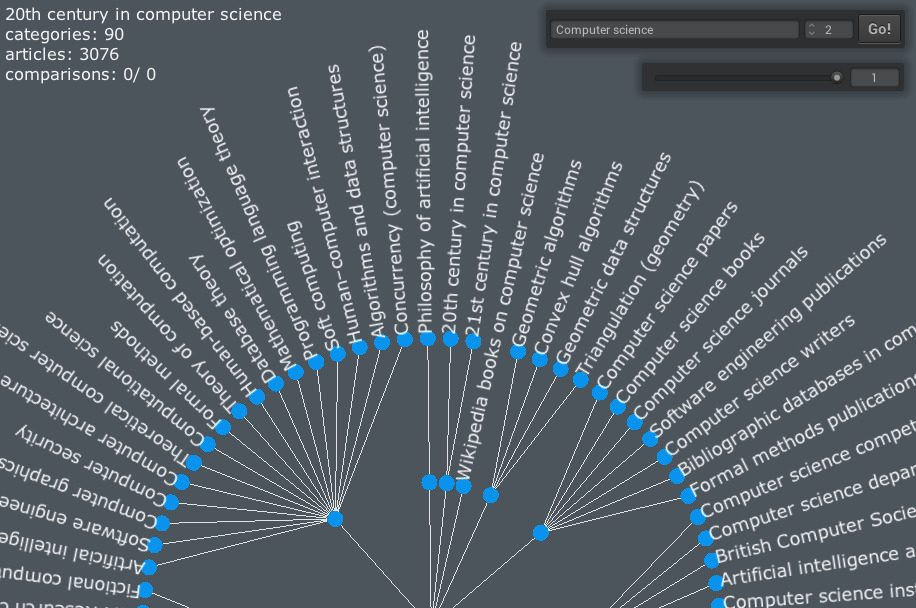
\includegraphics[width=\textwidth]{images/start-half}};
    \node[red, below] at (fig.south) {(a)};
    
    \node (one) at(-2.6,7.7) [rectangle, draw=red, very thick, inner sep=0pt, minimum width=5.2cm, minimum height=1.5cm]{};
    \node[red, below] at (one.south) {(b)};
    
    \node (two) at(7.85,7.9) [rectangle, draw=red, very thick, inner sep=0pt, minimum width=6.6cm, minimum height=.77cm]{};
    \node[red, above] at (4.5, 6.6){(c)};
    \node (three) at(8.75,7.1) [rectangle, draw=red, very thick, inner sep=0pt, minimum width=4.8cm, minimum height=.6cm]{};
    \node[red, below] at (three.south) {(d)};
    \end{tikzpicture}
    \caption{In der Darstellung der Kategorie \emph{Computer science} sind die Unterkategorien im Zentrum des radialen Graphen mit einer Tiefe von 1 mit der Stammkategorie verbunden und sichtbar.\\ (a) Hauptfenster, (b) zusammenfassende Statistik über vorhandene Daten, (c) Suchleiste, (d) Regler zur Änderung des Schwellwerts}
    \label{fig:small-start}
\end{figure}


\section{Layout} \label{subchap:layout}

In dieser Arbeit werden Ausschnitte der Kategorienstruktur der Wikipedia, welche sich insgesamt auf etwa $1.4$~Millionen Seiten beläuft, siehe die Tabelle \ref{tab:xml-overview}, dargestellt.
Wie einleitend in diesem Kapitel beschrieben, werden die Kategorien der Wikipedia in Form eines hierarchischen Baums modelliert.
Die Veränderung der Baumdarstellung durch das Hinzufügen von Knoten wird ebenfalls ermöglicht. 
Es gibt verschiedene Varianten, Bäume anzuordnen. 
Bekannte Methoden sind die horizontale und die vertikale Ausrichtung von Baumdarstellungen.
Die enorme Menge an möglichen Kategorien, die dargestellt werden sollen, erfordert eine Methode, welche den vorhandenen Platz des Computer-Bildschirms voll ausschöpft und dabei die Anordnung von Knoten in kurzer Zeit, also möglichst ohne Verzögerung, berechnet.
Hierfür werden wiederum zwei Ansätze getestet, welche nachfolgend erläutert werden.\\
Der erste Versuch wird mit dem Algorithmus nach Fruchtermann et al. \cite{fruchterman1991graph} implementiert.
Diese Arbeit verwendet eine Implementierung des Algorithmus aus der \emph{Boost Graph Library} \footnote{\url{http://www.boost.org/doc/libs/1_65_1/libs/graph/doc/index.html}}. Die Standardeinstellungen der Parameter dieses Algorithmus werden beibehalten.
In diesem Versuch stellt sich heraus, dass die Berechnung der Knoten anhand eines physikalischen Modells ab einer gewissen Größe zu rechen- und zeitintensiv wird, sodass keine Interaktion mit der Darstellung möglich ist.
Ein weiteres Problem dieses Ansatzes ist die Positionierung der Knoten.
Aus der Anordnung der Knoten nach dem Algorithmus von Fruchtermann et al.~\cite{fruchterman1991graph} lässt sich die hierarchische Struktur der Kategorien nur schwer erkennen. 
Folglich ist der Algorithmus in dieser Form nicht optimal für die Darstellung des Kategorienbaums und wird deshalb in dieser Arbeit nicht weiter verfolgt.

Der zweite Ansatz versucht die Anordnung der Knoten des Kategorienbaums mit dem Algorithmus nach Eades \cite{eades1991drawing} zu realisieren.
Die Positionierung der Knoten erfolgt in einem polaren Koordinatensystem, dabei stellt die Wurzelkategorie den Ursprung dieses Systems dar.
Die Distanz und der Winkel zum Ursprung geben die Position eines Knotens an.
Der Algorithmus ermöglicht es, dass jegliche Knoten einer Baumdatenstruktur als Wurzel für die Darstellung gewählt werden können. Anhand des ausgesuchten Knotens werden alle anderen Knoten in konzentrischen Ringen um den Wurzelknoten angeordnet.
Die Größe eines Sektors innerhalb des polaren Koordinatensystems, welcher für einen Teilbaum belegt wird, ist davon abhängig, wie viele Knoten sich in dem Teilbaum befinden.
Ausschlaggebend für die Größe des Sektors ist dabei die Anzahl an Blattknoten des jeweiligen Teilbaums, siehe hierzu Eades \cite[S.~15]{eades1991drawing}.
Der Algorithmus garantiert, dass die Anordnung des Baumes planar ist, also keine Überlappungen entstehen. \cite[S.~16]{eades1991drawing}.
Der Algorithmus erfüllt zudem die oben beschriebenen Voraussetzungen zur Darstellung des Kategorienbaumes.

\begin{figure}[H]
    \centering
    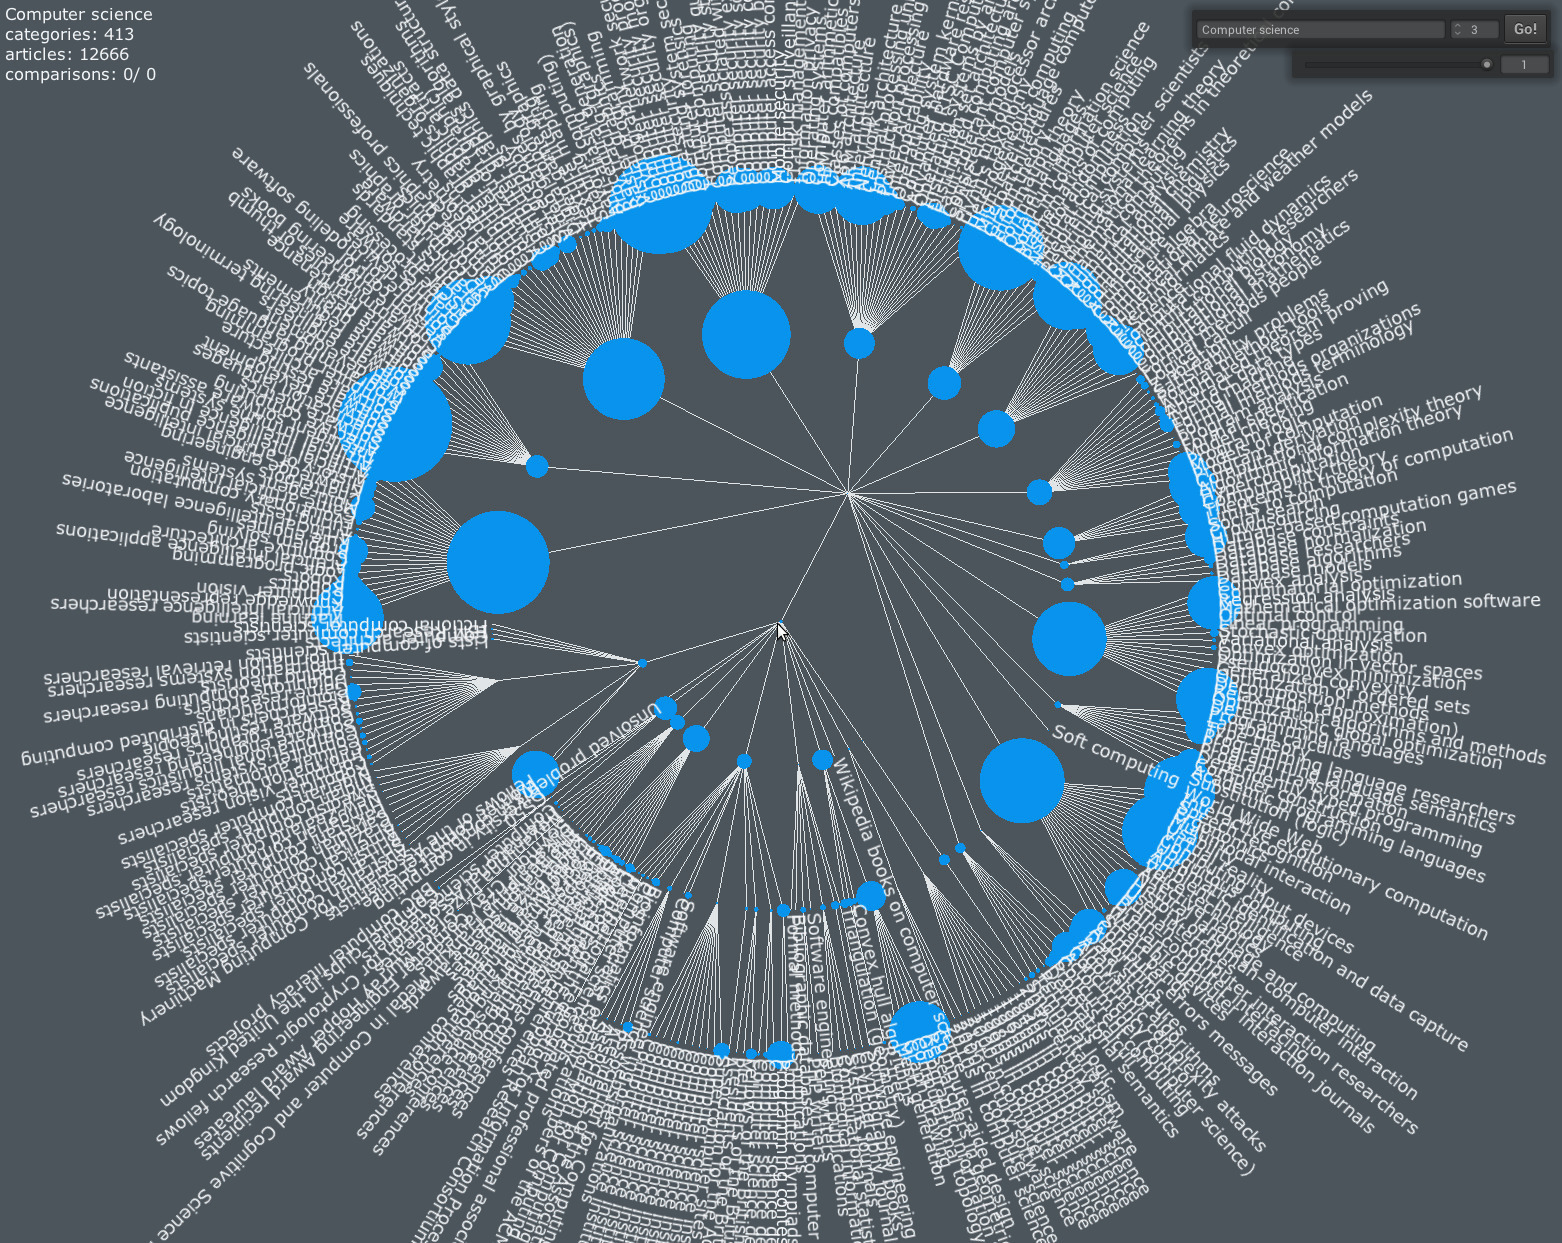
\includegraphics[width=\textwidth]{images/cat-size-direct}
    \caption{Die Anzahl der Artikel einer Kategorie wird direkt auf die Größe des Knotens der Kategorie übertragen}
    \label{fig:cat-size-direct}
\end{figure}


Im Folgenden werden die Merkmale für Kreisdarstellungen aus der Taxonomie von Kreisen nach \cite[S.~57]{lima2017circle} genutzt, um den dargestellten Baum zu erläutern.\\
Die Kategorien der Wikipedia werden als Knoten in Form von blau gefärbten Kreisen dargestellt.
Die Verbindungen zwischen den Wikipedia-Kategorien werden als Kanten in Form einer weißen Linie zwischen zwei Knoten dargestellt.
Nachfolgend wird der Begriff der Kategorie stellvertretend für die visuelle Form eines Knotens genutzt.
Die im Zentrum des Baums liegende Kategorie repräsentiert die Stammkategorie und wird auch Wurzelkategorie genannt.
Alle dargestellten Knoten sind durch Kanten mit ihr verbunden.\\
Kategorien, die keine Unterkategorien besitzen, werden Blattkategorien genannt.

Die Distanz zwischen zwei Kategorien wird durch die Anzahl an Kanten festgelegt, die auf dem kürzesten Pfad zwischen den beiden Kategorien liegen.
Die Distanz einer Kategorie zur Wurzelkategorie wird auch als Tiefe bezeichnet.
Die Unterkategorien der Wurzelkategorie werden auf konzentrischen Ringen um die Wurzelkategorie angeordnet, welche auch als Kategorienebene bezeichnet wird.
Alle Unterkategorien einer Kategorienebene besitzen die gleiche Distanz zur Wurzelkategorie.
Die Anzahl an konzentrischen Ringen wird durch die tiefste dargestellte Kategorie bestimmt.
In der Abbildung \ref{fig:small-start} wird die Visualisierung des Kategorienbaums mit einer Tiefe von 1 dargestellt.

Die Größe einer Kategorie wird an der Anzahl der direkten Artikel, die in der jeweiligen Kategorie eingetragen sind, gemessen.
Die Artikelanzahl kann direkt auf die Größe des Knotens der Kategorie übertragen werden, wie in der Abbildung~\ref{fig:cat-size-direct} dargestellt.
Jedoch ist dies nicht wünschenswert, da so ein Teil der Elemente des Kategorienbaums überzeichnet wird.
Es muss eine Darstellungsform gefunden werden, bei der die Größe der Knoten einen festgelegten Wert nicht überschreitet. 
In der Abbildung~\ref{fig:cat-size-fixed} wird dies dargestellt.
Der Unterschied in der Größe der Knoten soll dem Nutzer eine weitere grundlegende Information über die Kategorien liefern: die Artikelanzahl.
Dabei ist in der Abbildung~\ref{fig:cat-size-fixed} ebenfalls zu erkennen, dass es zu Irritationen führen kann, wenn die Wurzelkategorie nicht den größten Knoten darstellt.
Dies liegt daran, dass die Anzahl der Artikel nicht für die Unterkategorien einer Kategorie aufsummiert wird, da zuvor festgelegt wird, nur die direkten Artikel, welche in einer Kategorie eingetragen sind, zu zählen.

\begin{figure}[H]
    \centering
    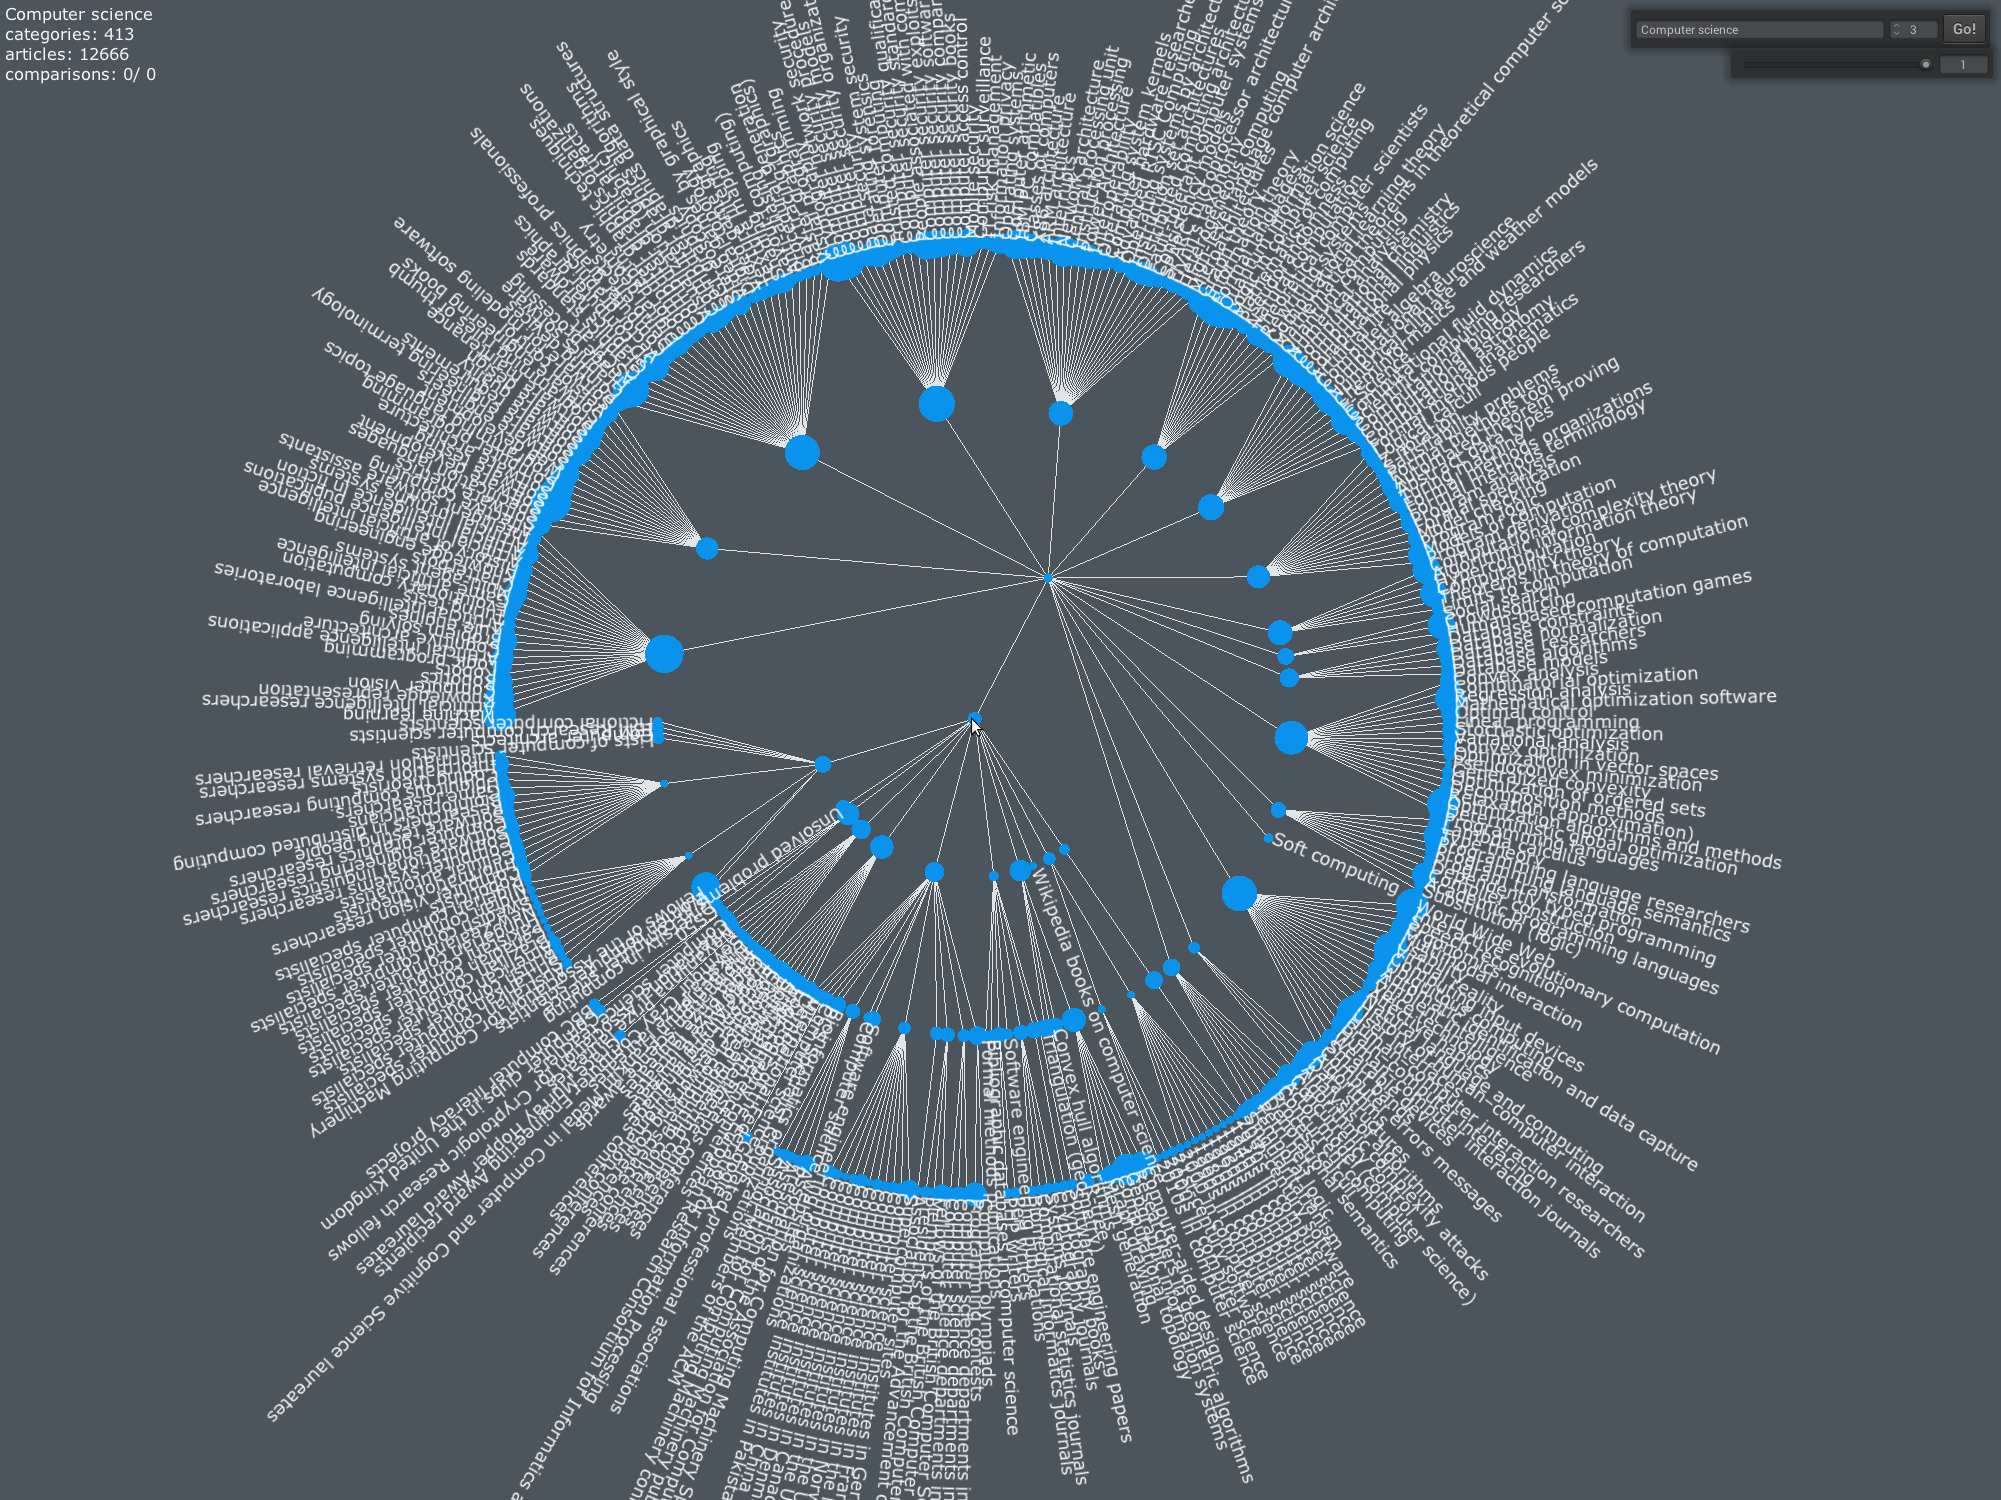
\includegraphics[width=\textwidth]{images/cat-size-fixed}
    \caption{Durch eine festgelegte Funktion wird die Anzahl der Artikel einer Kategorie auf einen Wert abgebildet, welcher den Durchmesser des Knotens darstellt.}
    \label{fig:cat-size-fixed}
\end{figure}

Die Beschriftung von Knoten ist notwendig, um die Knoten als Kategorien sichtbar zu machen und auch ohne die Interaktion von Seiten des Nutzers Informationen über den Kategorienbaum liefern zu können.
Die Beschriftung erfolgt dabei für alle Blattkategorien der Darstellung und erlaubt eine Untersuchung der benachbarten Kategorien.
Für den Fall, dass eine bestimmte Kategorie von Interesse ist und sie expandiert wird, werden ihre Unterkategorien beschriftet.
In dem Abschnitt~\ref{subchap:interaktion} wird die Interaktion durch eine Expansion im Detail beschrieben.\\
Die Titel werden im selben Winkel wie die jeweiligen Kategorien zum Ursprung angeordnet.
Die Anordnung der Titel einer Kategorie erfolgt gleich dem Winkel des Knotens der Kategorie.
Durch diese Anordnung sind Knoten mit einem Winkel über~90\textdegree{} und unter~270\textdegree{} schwer leserlich oder gar kopfüber angeordnet.
Deshalb beschreibt der Abschnitt~\ref{subchap:interaktion} eine Methode, welche die Lesbarkeit der Titel erleichtert.
% Die Wurzelkategorie im Zentrum des Kategorienbaums stellt dabei die gesuchte Kategorie 
% Lima beschreibt zwölf wesentliche Merkmale von Kreisen, dabei gehen wir nur auf Merkmale ein, die eine zentrale Rolle in der Visualisierung einnehmen.


\section{Interaktion} \label{subchap:interaktion}
Die folgenden Interaktionen werden am Beispiel eines stationären Rechners erläutert.
Dabei sind die Eingabegeräte die Maus und die Tastatur, das Ausgabegerät ist der Bildschirm.
% Für eine Anwendung auf anderen Geräten, wie einem \emph{Tablet} oder einem hochauflösenden \emph{Visual-Analytics-Display} sind andere Eingabemethoden notwendig.

Die Interaktionen mit der Visualisierung lassen sich in zwei Gruppen einteilen: Ein Nutzer kann entweder mit der grafischen Benutzeroberfläche interagieren, wie in der Abbildung~\ref{fig:small-start} mit~(b), (c) und~(d) markiert oder er interagiert direkt mit den Inhalten im Hauptfenster, wie in der Abbildung mit~(a) gekennzeichnet.
Nachfolgend werden diese Möglichkeiten zur Interaktion erläutert.

\paragraph{Grafische Benutzeroberfläche}
Das Element~(b) aus der Abbildung~\ref{fig:small-start} ist ein passives Interaktionselement, da es Informationen anzeigt, die nicht direkt durch den Nutzer verändert werden können.
Das Element besteht aus vier Zeilen, welche Informationen über den aktuellen Kategorienbaum innerhalb des Hauptfensters~(a) zur Verfügung stellen.
In der ersten Zeile wird der Titel der letzten Kategorie angezeigt, über welche der Nutzer den Mauszeiger platziert hat.
Hierdurch wird die Option geschaffen, Titel unbeschrifteter Kategorien zu erfahren.
Die zweite und dritte Zeile zeigen die Anzahl der Kategorien sowie die Anzahl der Artikel des dargestellten Kategorienbaums an.
Es werden hierbei alle Artikel gezählt, welche direkt in den Kategorienseiten eingetragen sind. Artikel, die mehrfach in unterschiedlichen Kategorien vorkommen, werden nur einmal berücksichtigt.
Die letzte Zeile des Elements~(b) beschreibt die Anzahl an Artikelpaaren, die über dem festgelegten Schwellwert aus Element~(d) liegen.
Die erste Zahl stellt dabei die Anzahl an Artikelpaaren dar, von denen beide Artikel einer Kategorie angehören, die auch im dargestellten Kategorienbaum zu finden ist.
Die zweite Zahl hingegen beschreibt solche Artikelpaare, in denen nur einer der beiden Artikel in einer Kategorie des Kategorienbaums dargestellt wird.
Diese zwei Varianten von Artikelpaaren werden im Rahmen dieser Arbeit \emph{lokale} bzw. \emph{globale} Vergleiche von Artikeln genannt.
Auf dieses Konzept wird in dem Abschnitt~\ref{subchap: filter-vis} eingegangen.

Das Element~(c) aus der Abbildung \ref{fig:small-start} ist Teil der grafischen Benutzeroberfläche und dient als Suchleiste für sämtliche Kategorien der Wikipedia.
Die Suchleiste ist dabei aus drei Elementen aufgebaut, wie in der Abbildung~\ref{fig:searchbar} dargestellt: dem Suchformular~(1), dem Eingabefeld für die Tiefe~(2) und der Schaltfläche~(3).

\begin{figure}
    \centering
    \begin{tikzpicture}
        \node (fig) at (0,0) {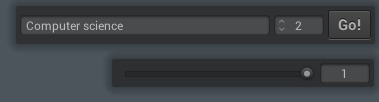
\includegraphics[scale=.8]{images/searchbar}};

        \node (one) at(-1.3,0.7) [rectangle, draw=red, very thick, inner sep=0pt, minimum width=7.1cm, minimum height=1.0cm]{};
        \node[red, below] at (one.south) {(1)};
        \node (two) at(3.1,0.7) [rectangle, draw=red, very thick, inner sep=0pt, minimum width=1.5cm, minimum height=1.0cm]{};
        \node[red, below] at (two.south) {(2)};
        \node (three) at(4.6,0.7) [rectangle, draw=red, very thick, inner sep=0pt, minimum width=1.3cm, minimum height=1.0cm]{};
        \node[red, below] at (three.south) {(3)};
     
    \end{tikzpicture}
    \caption{Darstellung der Suchleiste und des Reglers für den Schwellwert.}
    \label{fig:searchbar}
\end{figure}

In der Suchleiste kann der Name einer möglichen Kategorie als Suchbegriff eingegeben werden.
Betätigt der Nutzer nach der Eingabe einer gesuchten Kategorie die Schaltfläche "`Go!"', wird eine Suchanfrage mit dem eingegebenen Begriff an die Datenbank weitergeleitet.
Existiert keine Kategorie mit dem eingegebenen Begriff, wird die Schaltfläche "'Go!"` rot eingefärbt und der Nutzer aufgefordert, eine andere Kategorie einzugeben, siehe die Abbildung~\ref{fig:wrong-cat}.

\begin{figure}[H]
    \centering
    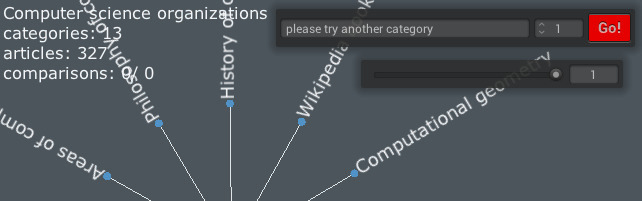
\includegraphics[scale=.5]{images/wrong-cat-small}
    \caption{Der Nutzer suchte nach einer Kategorie, welche nicht in der Datenbank gefunden wird. Der Nutzer wird durch die grafische Benutzeroberfläche dazu aufgefordert, die Suche zu wiederholen.}
    \label{fig:wrong-cat}
\end{figure}

Existiert die Kategorie allerdings in der Datenbank, wird ein Kategorienbaum nach den festgelegten Parametern gezeichnet.
Der im Eingabefeld eingetragene Tiefen-Wert legt dabei die Anzahl der Ebenen fest.
Die gesuchte Kategorie wird zum Zentrum der Darstellung.

Das Feld für die Tiefe des Kategorienbaums kann durch die Eingabe des Nutzers verändert werden.
Die Eingabe einer Zahl wird durch die Tastatur oder über die Pfeile im Eingabefeld ermöglicht.
Mit dem Tiefen-Wert wird die maximale Tiefe des Kategorienbaums, bis zu welcher die Blattkategorien expandiert werden sollen, festgelegt.
Sollten Unterkategorien mit einem höheren Tiefenwert in der Darstellung angezeigt werden, betrifft sie diese Interaktion nicht.
Demzufolge ist die Distanz zwischen Blattkategorien und der Wurzelkategorie mindestens so groß wie die eingegebene Tiefe.
Die Expansion der Blattkategorien wird durch Betätigung der Schaltfläche "`Go!"' ausgeführt.
Dabei bleiben bereits gezeichnete Kategorien der Visualisierung unverändert, sofern sie tiefer als die Eingabetiefe sind.

Das andere Element der grafischen Benutzeroberfläche ist der Regler, mit dem ein Schwellwert für Ähnlichkeiten festgelegt wird.
Dieser wird in der Abbildung~\ref{fig:small-start} mit~(d) gekennzeichnet.
Das Element besteht aus zwei Feldern, einem Schieberegler und einem Zahlenfeld, an dem der eingestellte Wert abgelesen werden kann.
Der Schieberegler stellt dabei eine Mindestgröße ein, die den Ähnlichkeitswert zwischen zwei Artikeln überschreiten muss, um dargestellt werden zu können.
Artikelpaare mit einem Ähnlichkeitswert, der niedriger ist als der Schwellwert, werden nicht in Betracht gezogen.
% Die Veränderung des Schiebereglers ändert neben dem Schwellwert auch die Farbe der Knoten von blau nach gelb.
Der Schieberegler beeinflusst nicht nur die Selektion der Daten aus der Ähnlichkeitsmatrix, sondern auch das Erscheinungsbild der Visualisierung.
Kategorien werden gelb gefärbt, wenn die darin eingetragenen Artikel eine Ähnlichkeit zu einem Artikel aus einer bereits dargestellten Kategorie aufweisen, die höher oder gleich dem Schwellwert ist.
Der Schieberegler zeigt folglich die Kategorien an, unter denen Artikelpaare mit einer Ähnlichkeit über oder gleich dem Schwellwert eingetragen sind.
Diese Form der Selektion einer dünn besetzten Ähnlichkeitsmatrix wird in dieser Arbeit horizontale Filterung bezeichnet.
Die Abbildung~\ref{fig:simM-threshold-cat} verdeutlicht dies.

\paragraph{Hauptfenster}
Als Hauptfenster wird der Bereich bezeichnet, der in der Abbildung~\ref{fig:small-start} mit~(a) markiert ist.
Im Hauptfenster wird der Kategorienbaum als Knoten- und Kantendiagramm dargestellt.
Der Kategorienbaum steht im Mittelpunkt der Visualisierung.
Es bestehen verschiedene Möglichkeiten, mit dem Kategorienbaum zu interagieren:
\begin{enumerate}[label*=(\arabic*),leftmargin=1.5cm,series=example]
\item{die Verschiebung und das Vergrößern}
\item{die Rotation}
\item{die Erweiterung des Kategorienbaums}
\end{enumerate}
\begin{figure}[H]
    \centering
    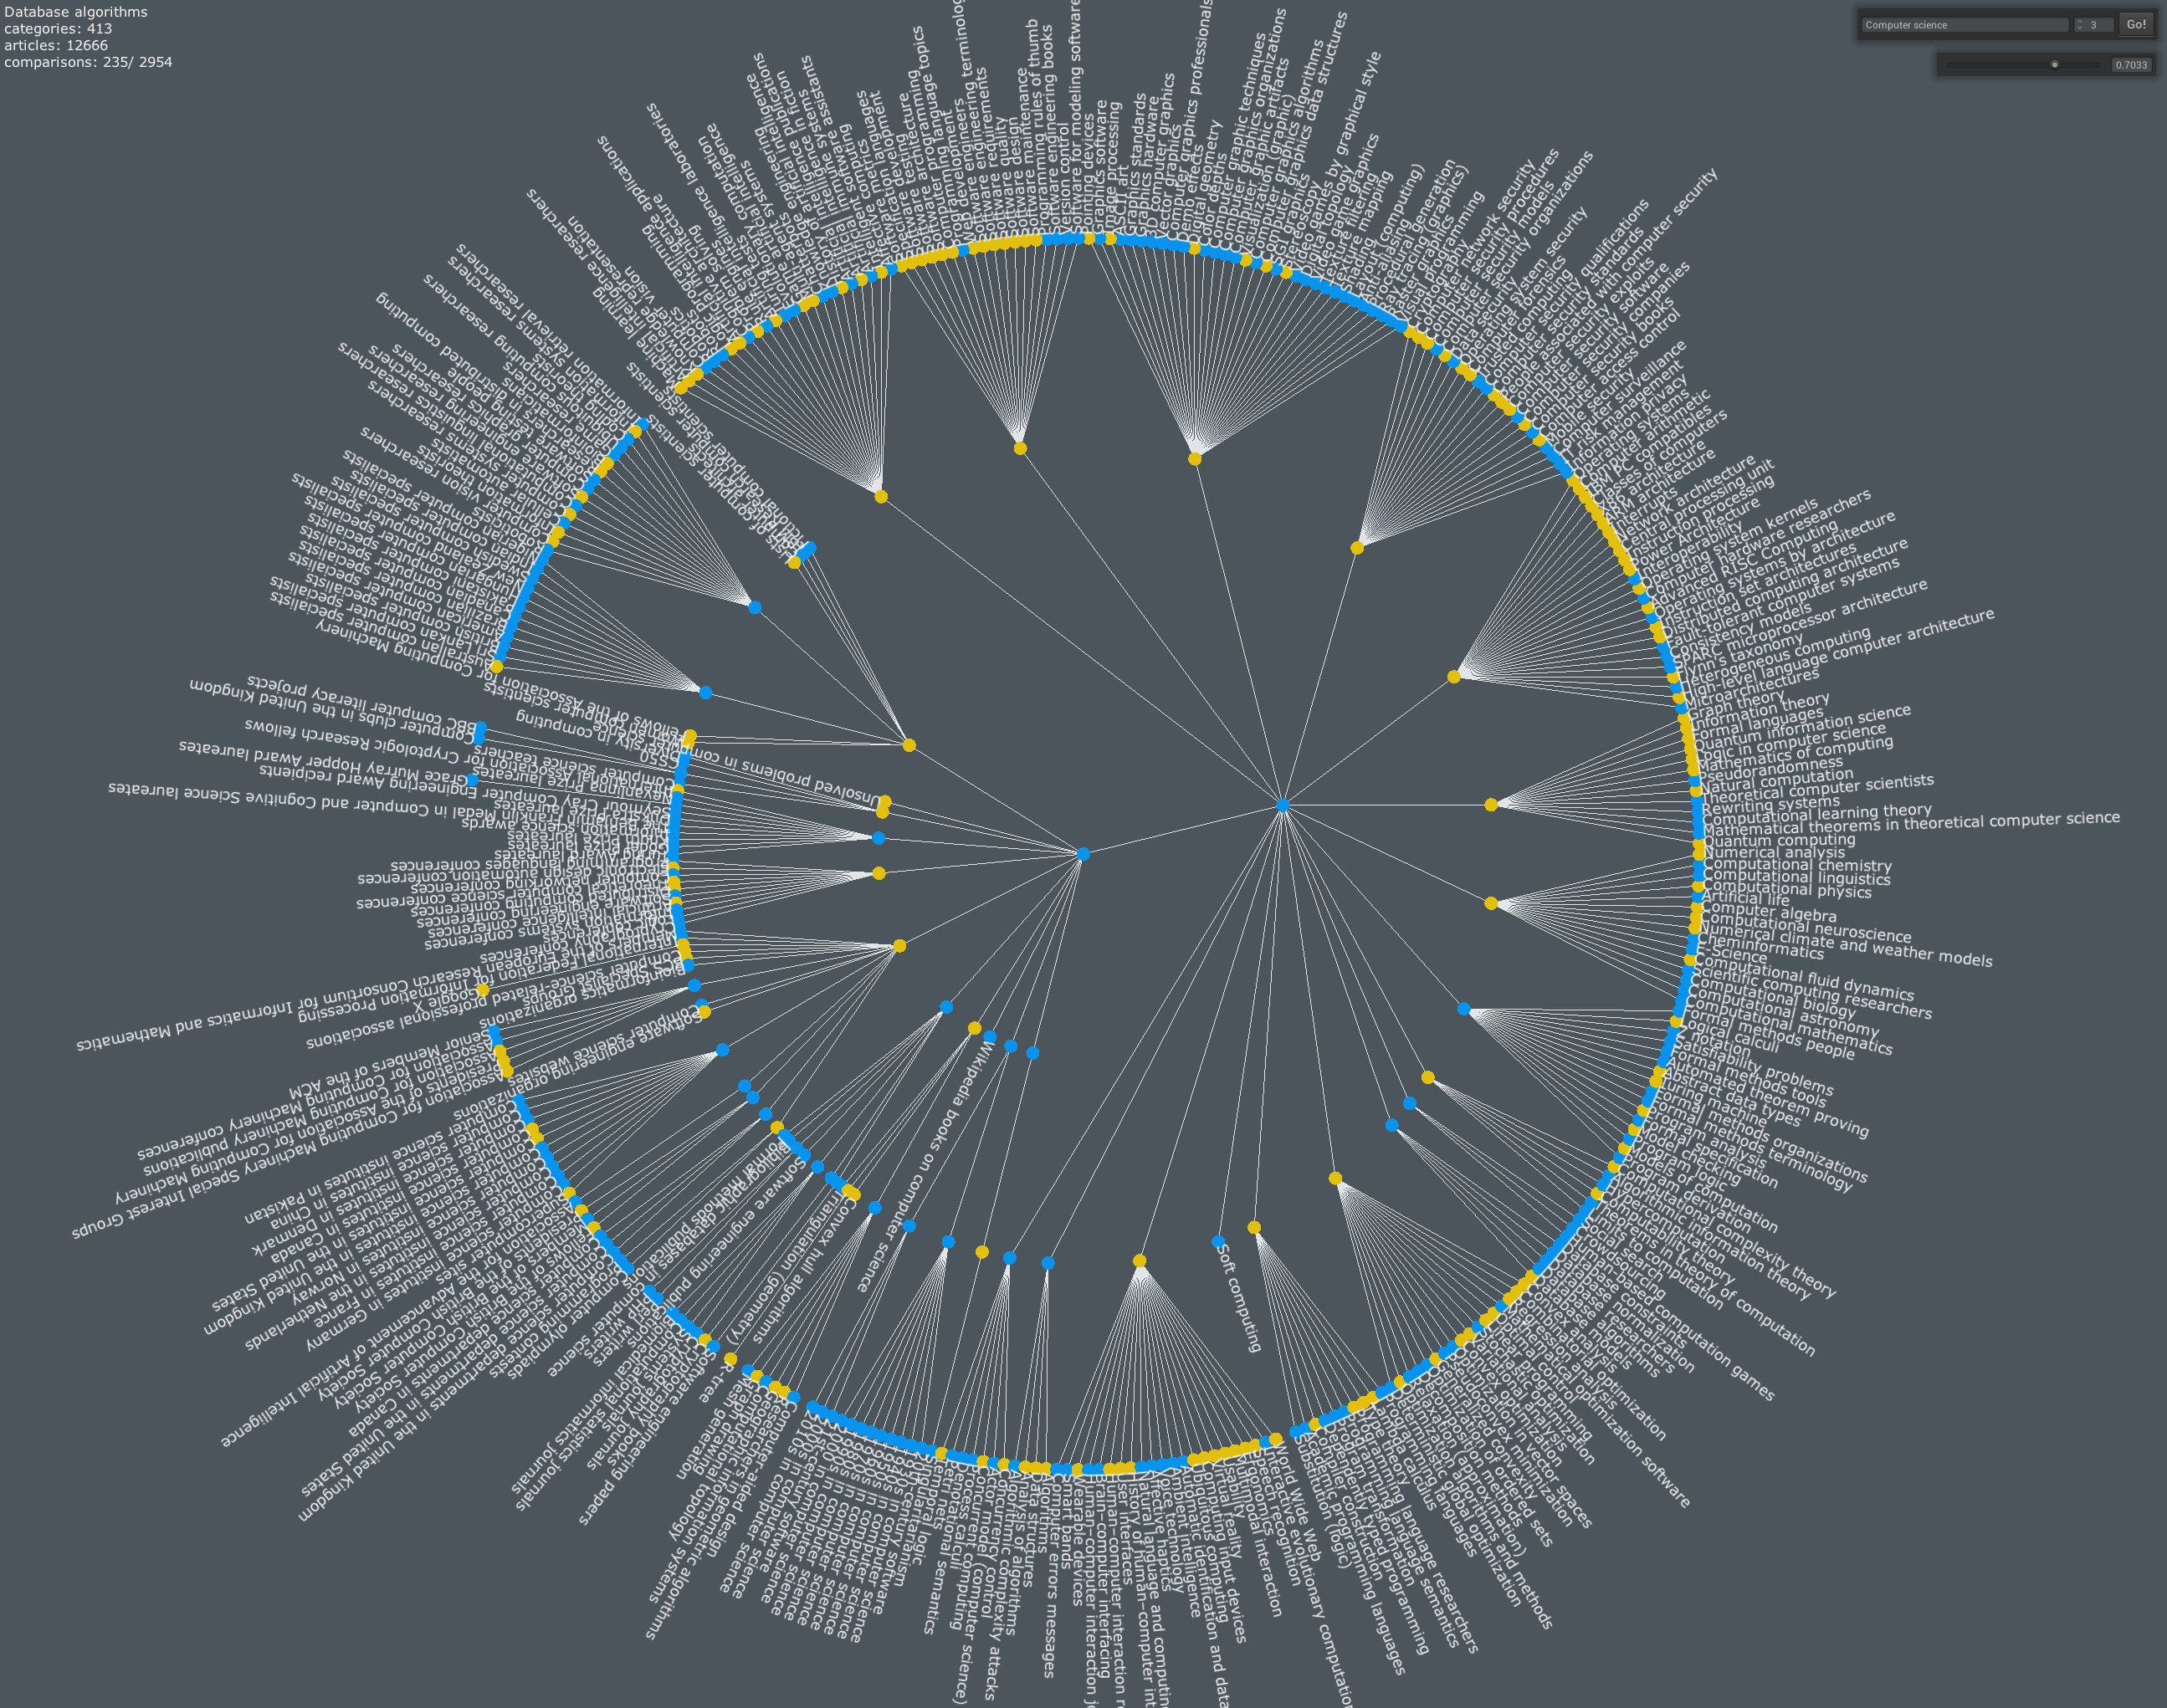
\includegraphics[width=\textwidth]{images/filter-7033}
    \caption{Die Färbung von Kategorien über dem Schwellwert und die Eingabe des Schwellwerts}
    \label{fig:simM-threshold-cat}
\end{figure}


Durch die Verschiebung und die Vergrößerung der Darstellung des Kategorienbaums wird dem Nutzer die Möglichkeit gegeben, den Kategorienbaum frei zu platzieren und ausgewählte Knoten zu fokussieren.
Durch die radiale Anordnung der Kategorien und ihre Beschriftung in radialer Ordnung ist es möglich, den Kategorienbaum um die Wurzelkategorie zu drehen.
Bei gedrückt gehaltener "`Strg"'-Taste und gleichzeitiger Drehung am Mausrad dreht sich auch der Kategorienbaum.
Diese interaktive Funktion soll dem Nutzer ermöglichen, den Kategorienbaum so ausrichten zu können, dass er im Stande ist, die Beschriftung einer bestimmten Kategorie zu lesen.
\begin{figure}
    \centering
    \begin{tikzpicture}
    \matrix (m) [matrix of nodes, nodes in empty cells]
    {
        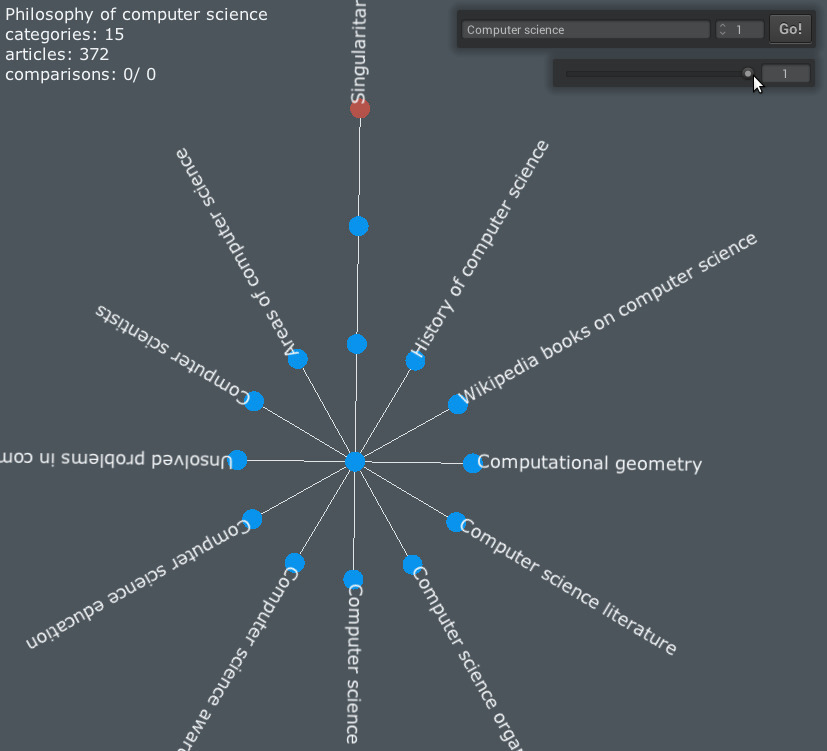
\includegraphics[scale=.18 ]{images/rotation-1}&[3mm]&
        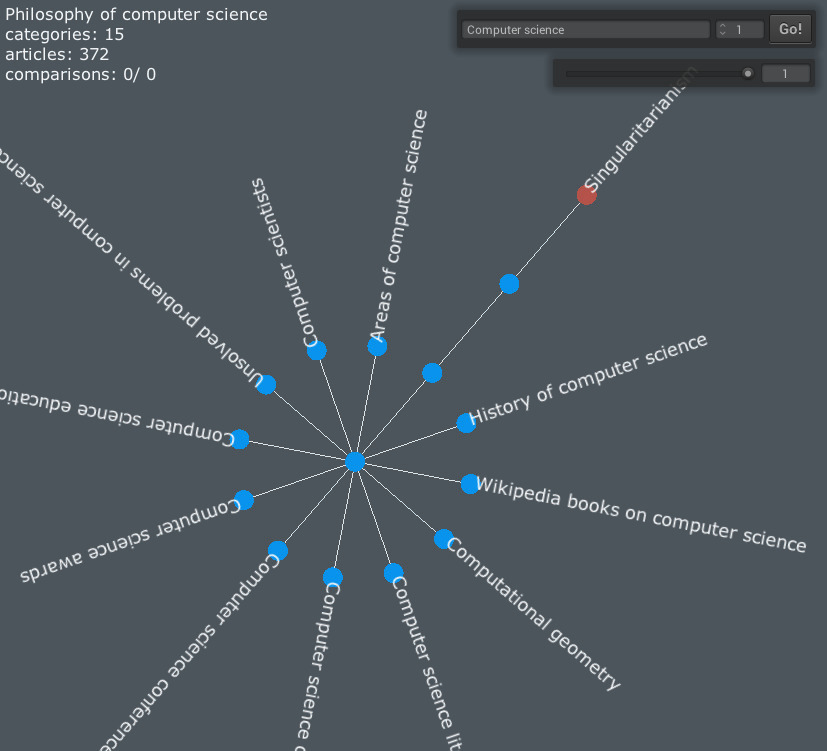
\includegraphics[scale=.18 ]{images/rotation-2}&[3mm]&
        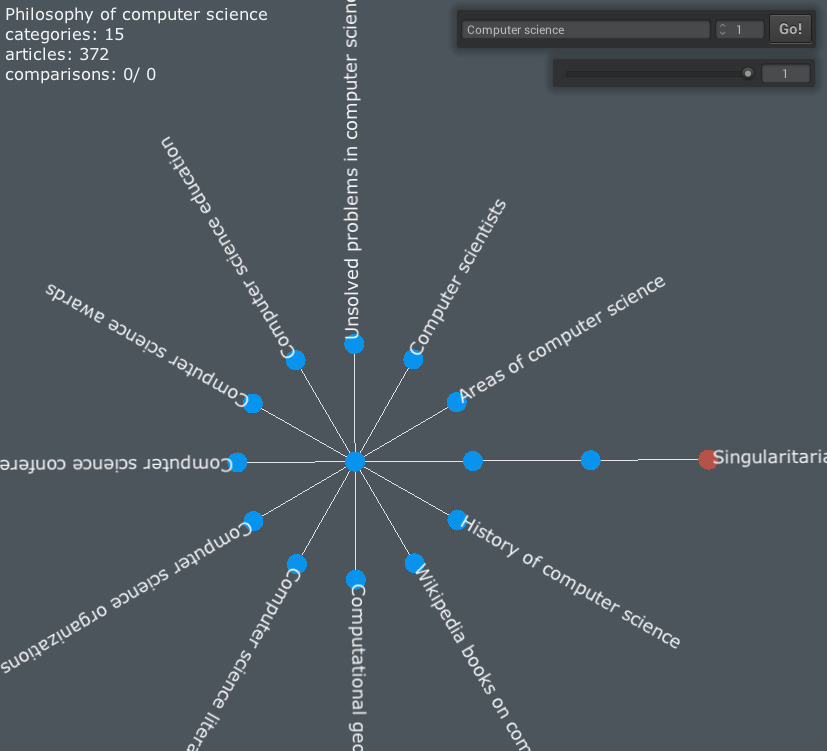
\includegraphics[scale=.18 ]{images/rotation-3}\\
    };
    \draw[-{Latex[length=3mm]}] (m-1-1) -- (m-1-3);
    \draw[-{Latex[length=3mm]}] (m-1-3) -- (m-1-5);
    \end{tikzpicture}
    \caption{Der Kategorienbaum für die Wurzelkategorie \emph{Computer science} wird um~90\textdegree Grad im Uhrzeigersinn gedreht. Der Pfad der Unterkategorie\emph{Philospohy of computer science} ist expandiert.}
    \label{fig:rotation-tree}
\end{figure}

% zwei Bilder mit Pfeil Drehung der Kategorie
Platziert der Nutzer den Mauszeiger über einer bestimmten Kategorie, wird ihm deren Titel in der zusammenfassenden Statistik angezeigt. Dies ist in der Abbildung~\ref{fig:small-start} zu erkennen.
Somit ist es auch möglich, sich Titel von Kategorien, die keine Blattkategorien sind, anzeigen zu lassen, ohne dass sich die gezeichneten Elemente überlagern.

Die grundlegende Interaktion mit der Visualisierung ist die Expansion ausgewählter Kategorien.
Diese Erweiterung einer Kategorie wird durch einen Doppelklick auf die Kategorie ausgeführt.
Dabei werden die Unterkategorien der Ausgangskategorie dem Kategorienbaum hinzugefügt und als Knoten in die Visualisierung gezeichnet.
Die neuen Unterkategorien werden durch Kanten mit der Ausgangskategorie verbunden.
Dies wird in der Abbildung~\ref{fig:expand-cat} verdeutlicht.
Die Expansion ermöglicht dem Nutzer, einen bestimmten Pfad von Unterkategorien schrittweise zu erkunden.
Die Erkundung der Unterkategorien eines Themengebietes wird dadurch differenzierter. 
Neben der Expansion des Kategorienbaums für alle Blattkategorien durch das Eingabefeld für die Tiefe wird zudem die Voraussetzung für eine feinere Interaktion geschaffen.
Die Erweiterung einer Kategorie ist als eine inhaltliche Vertiefung zu verstehen.
Das Hinzufügen von Unterkategorien zum Kategorienbaum stellt eine Spezifizierung des umschriebenen Gegenstands der Ausgangskategorie dar.
Diese Spezifizierung des umschriebenen Gegenstandes durch die Unterkategorien wird in dieser Arbeit als inhaltliche Vertiefung festgelegt.
Die Expansion stellt dabei immer eine Spezifizierung der Abstraktionsebene dar, da dem Kategorienbaum nur Unterkategorien hinzugefügt werden können.

\begin{figure}[H]
    \centering
    \begin{tikzpicture}
    \matrix (m) [matrix of nodes, nodes in empty cells]
    {
        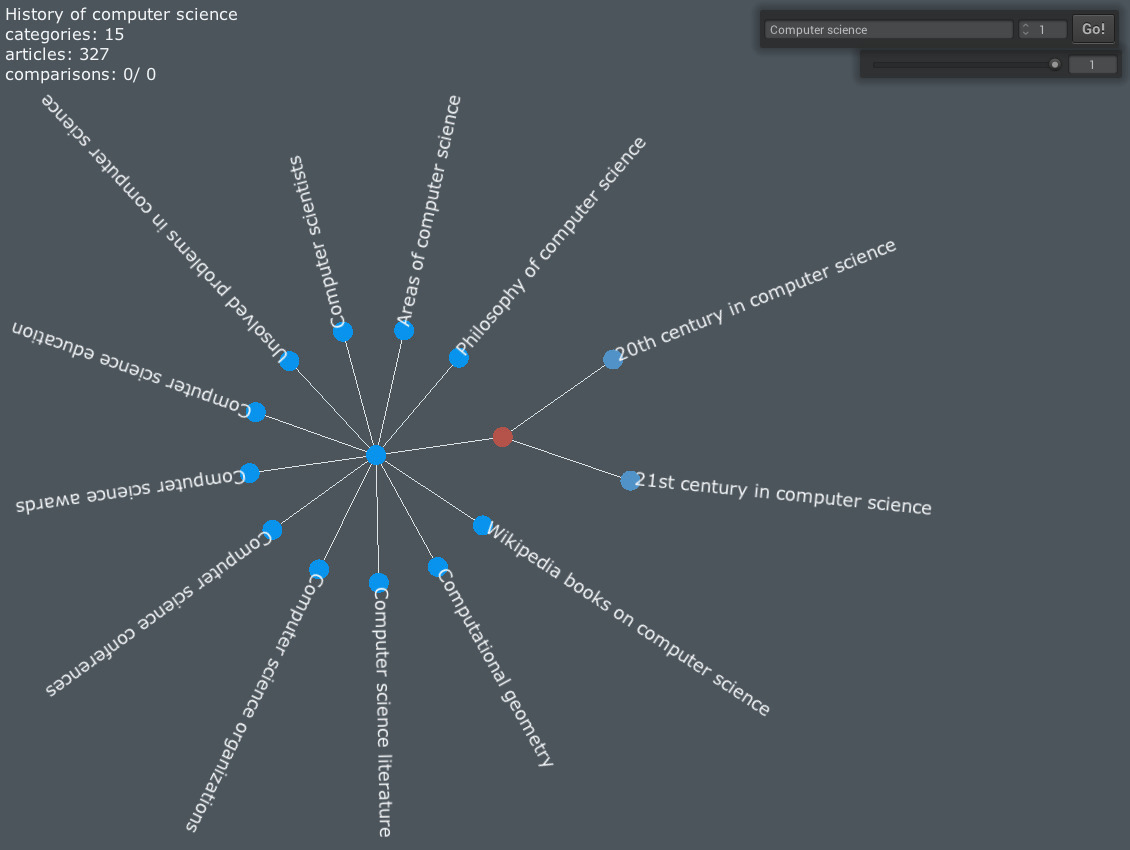
\includegraphics[scale=.18 ]{images/expand-1}&[3mm]&
        % 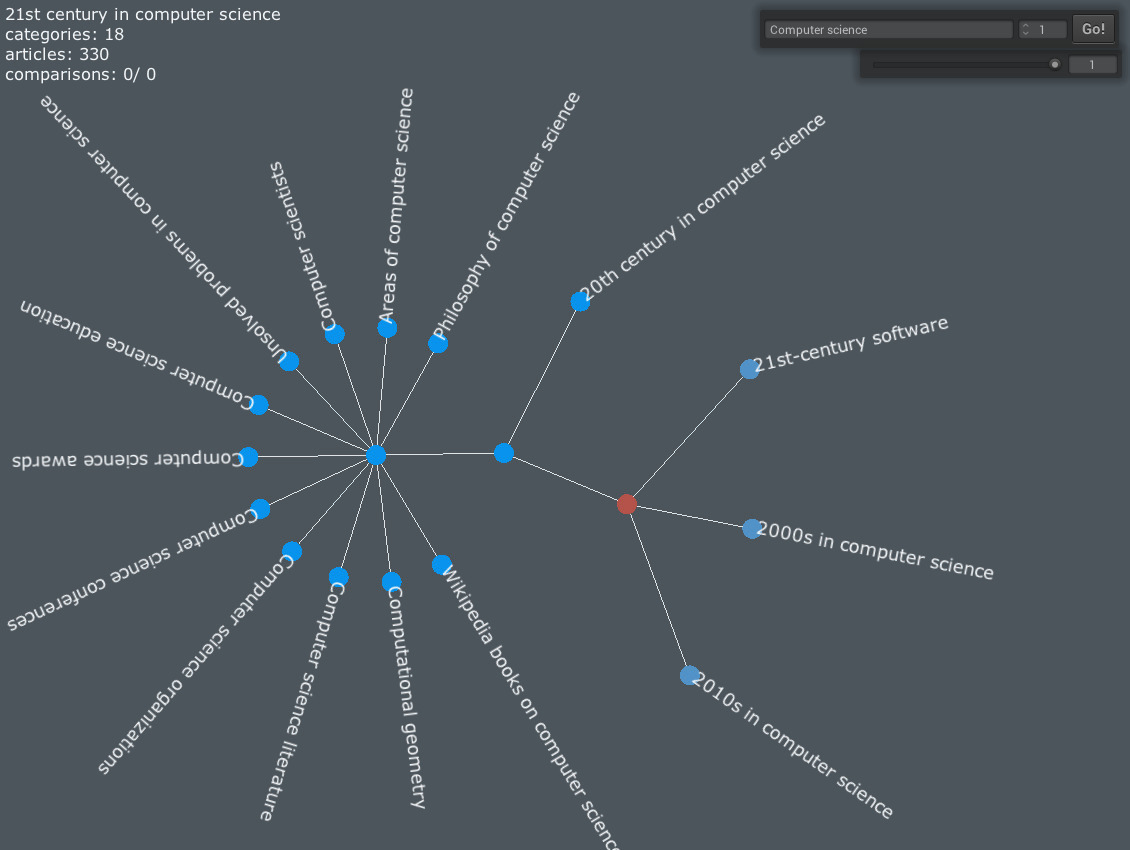
\includegraphics[scale=.18 ]{images/expand-2}&[3mm]&
        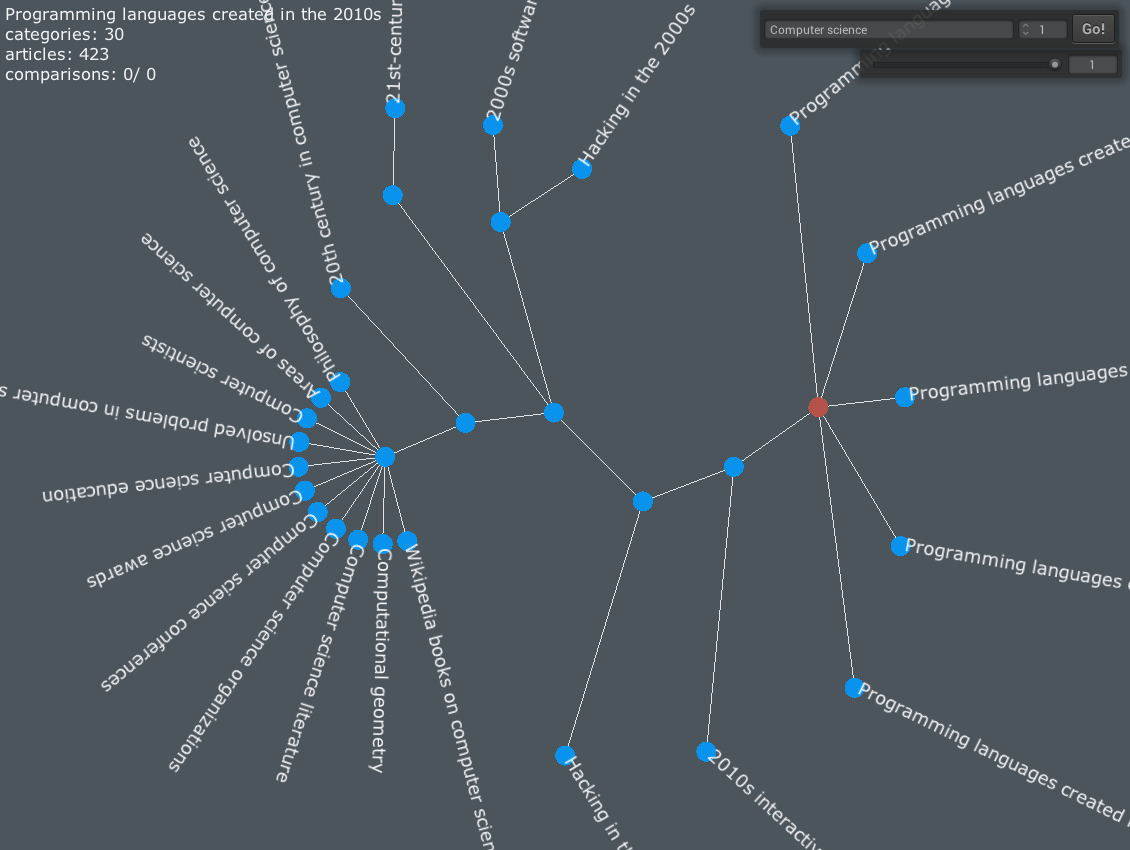
\includegraphics[scale=.18 ]{images/expand-3}\\
    };
    \draw[-{Latex[length=3mm]}] (m-1-1) -- (m-1-3);
    % \draw[-{Latex[length=3mm]}] (m-1-3) -- (m-1-5);
    \end{tikzpicture}   % \end{tikzpicture}
    \caption{Die Bildabfolge stellt mehrere Erweiterungen von Unterkategorien der Kategorie \emph{History of Computer Science} dar. Die zuletzt expandierten Kategorie ist rot gefärbt.}
    \label{fig:expand-cat}
\end{figure}

Mit einem Klick auf eine Kategorie wird die Kategorie rot gefärbt, damit diese von anderen Kategorien unterschieden werden kann.
Diese Auswahl einer Kategorie ergibt in Kombination mit der Änderung des Schwellwerts eine neue Interaktion.
Durch die Fokussierung einer Kategorie werden andere Kategorien nur dann gelb gefärbt, wenn sie folgende zwei Bedingungen erfüllen:
\begin{enumerate}[label*=(\arabic*),leftmargin=1.5cm,series=example]
\item{In der jeweiligen Kategorie existiert mindestens ein Artikel, der mit mindestens einem Artikel aus der ausgewählten Kategorie verglichen wurde}
\item{Der Ähnlichkeitswert liegt über dem definierten Schwellwert}
\end{enumerate}
Dieser Zustand wird in der Abbildung~\ref{fig:threshold-focus-cat} dargestellt.

\begin{figure}[H]
    \centering
    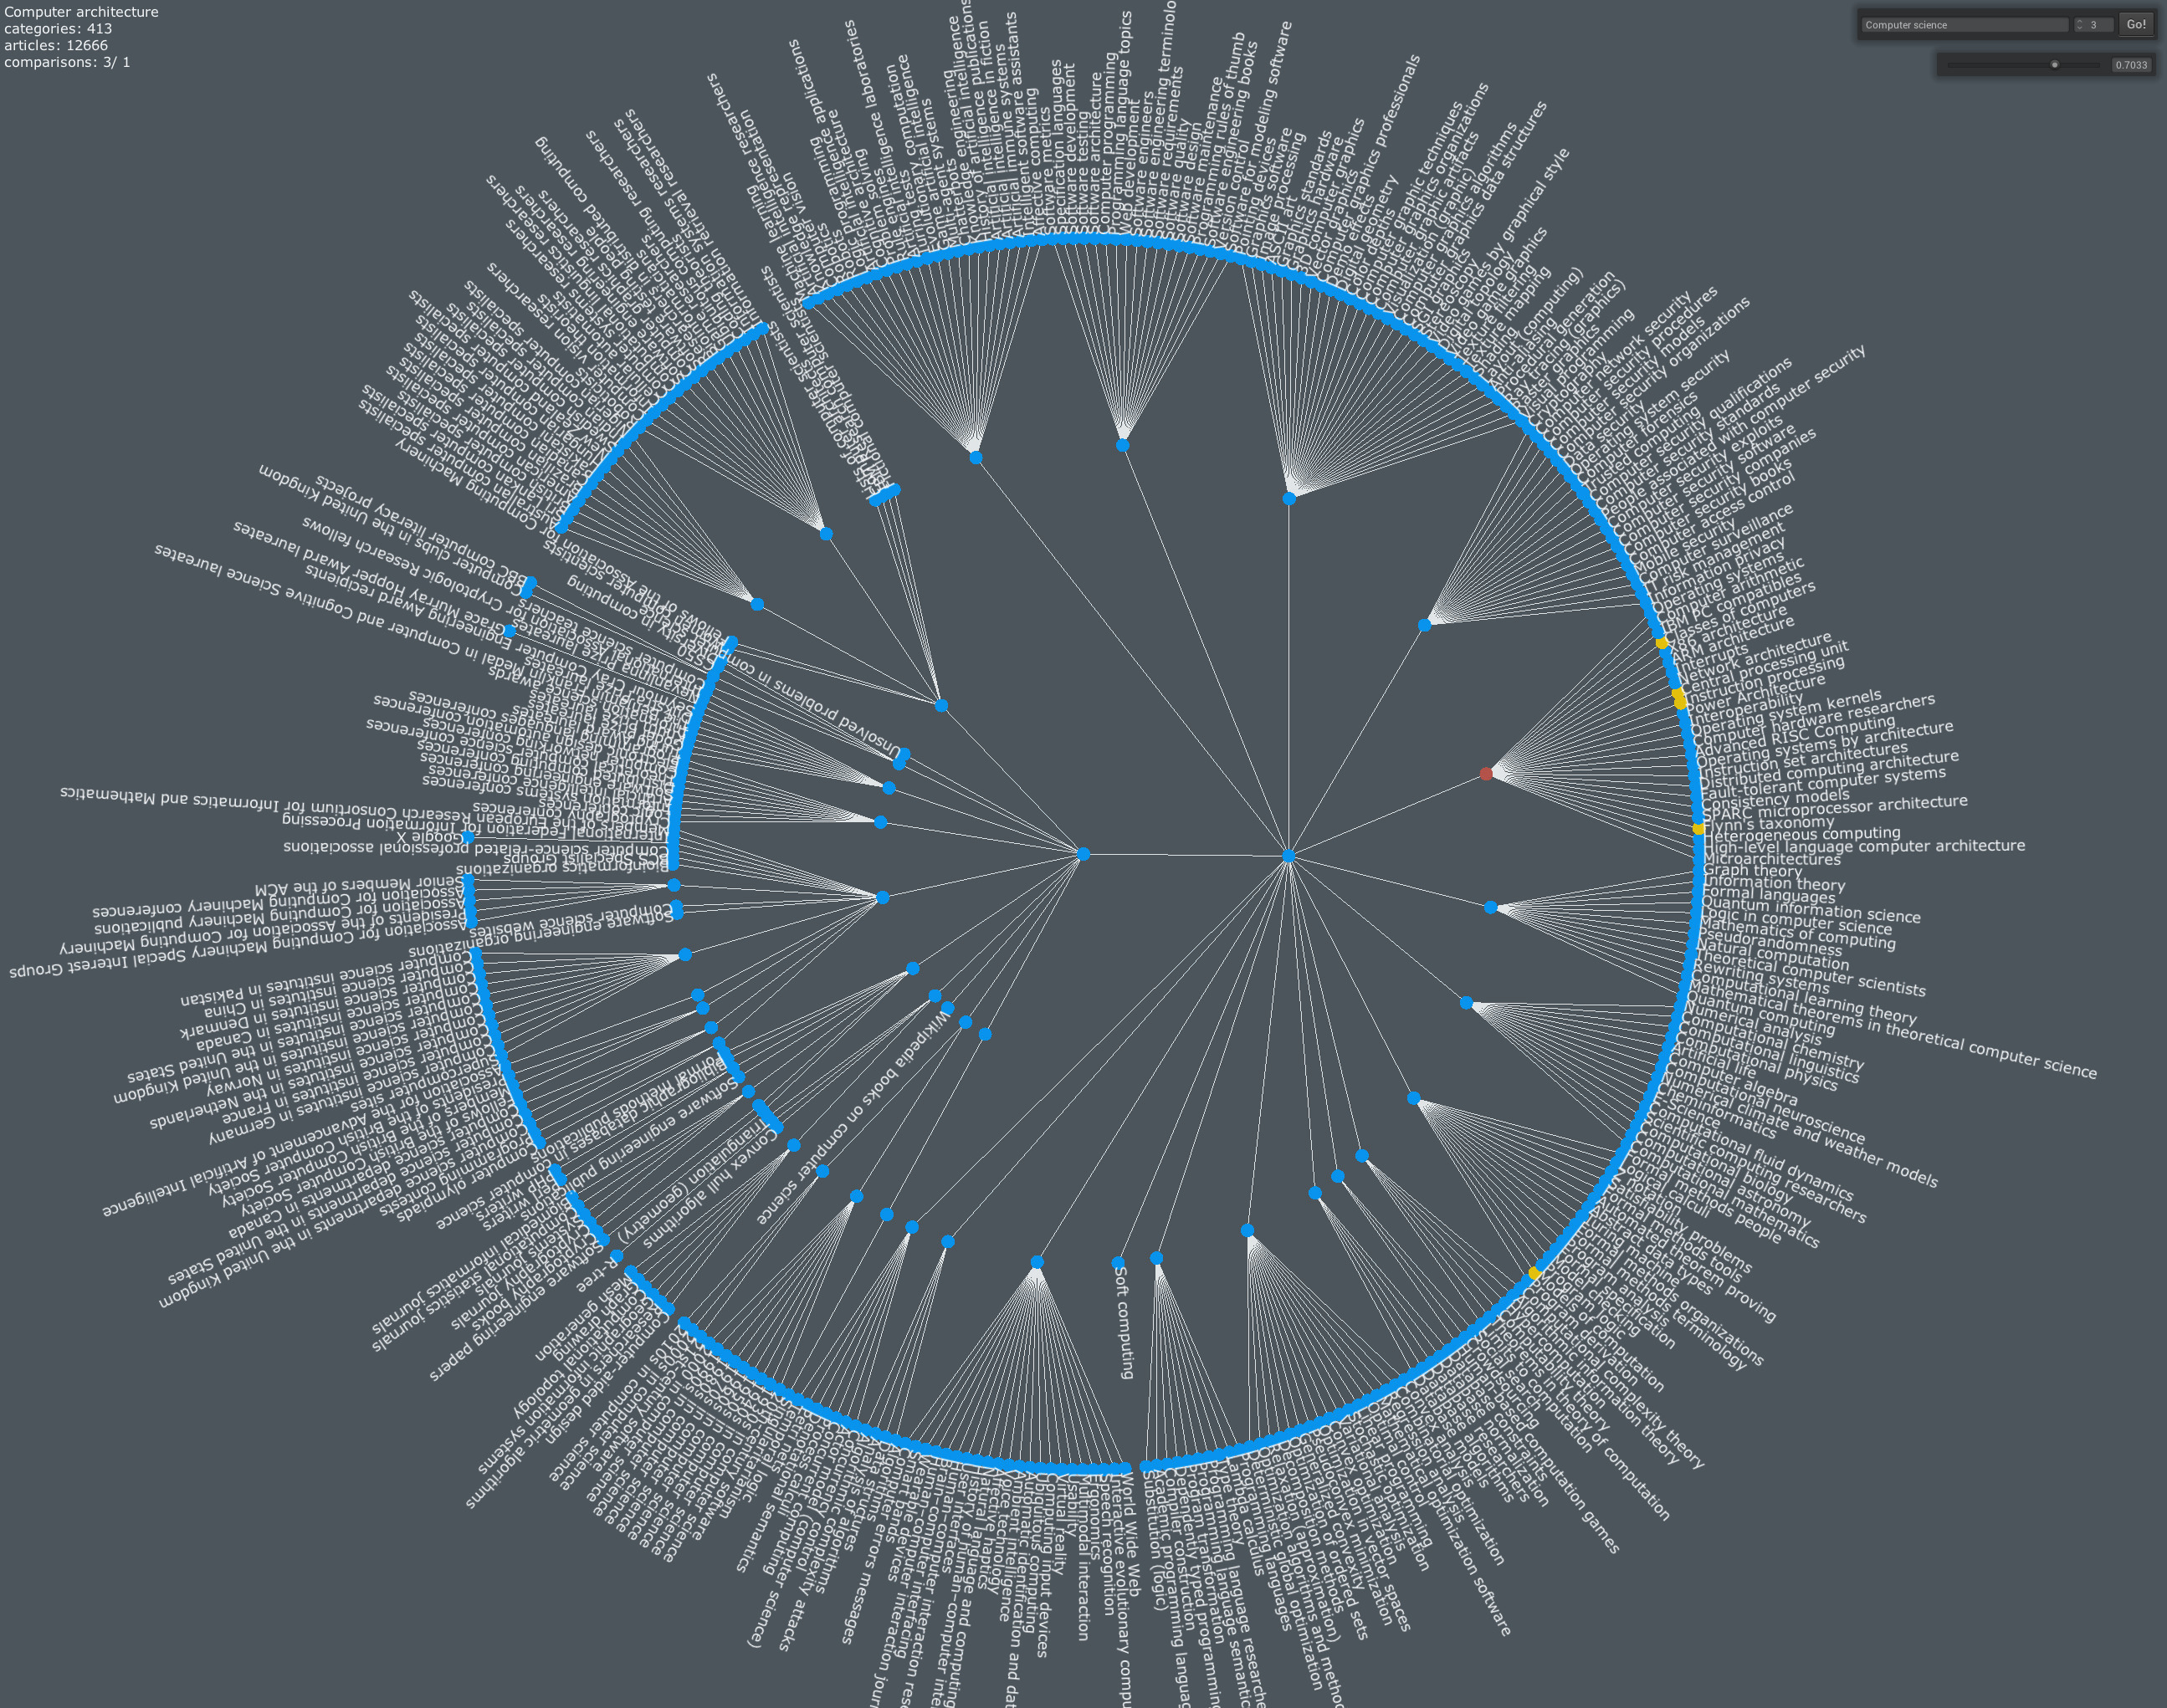
\includegraphics[width=\textwidth]{images/filter-7033-focus}
    \caption{Die rot gefärbte Kategorie \emph{Computer architecture} wurde fokussiert. In den gelb gefärbten Kategorien sind Artikel mit einer Ähnlichkeit zur rot gefärbten Kategorie eingetragen. Der Ähnlichkeitswert eines Artikelpaares zwischen zwei Kategorien liegt mindestens bei~$0.7033$.}
    \label{fig:threshold-focus-cat}
\end{figure}


\section{Filterung der "Ahnlichkeitsmatrix} \label{subchap: filter-vis}

% In diesem Abschnitt soll die Grafik über die simMatrix als abstraktes, nicht sichtbares Datenmodell dargestellt werden!!!
Dieses Kapitel beschäftigt sich damit, dass durch die Interaktion mit der Darstellung eine neue themenbezogene Ähnlichkeitsmatrix, wie in Kapitel~\ref{subchap:simmatrix} dargelegt, konstruiert wird.
Wie in der Einleitung dieses Kapitels bereits erwähnt, kann der Kategorienbaum als Hierarchie von Abstraktionsebenen interpretiert und die Exploration von Kategorien nach einer \emph{Top-Down}-Herangehensweise realisiert werden.
Für die Dauer einer Darstellung des Kategorienbaums werden auch die Informationen über Ähnlichkeiten von Artikeln aus der Ähnlichkeitsmatrix verfügbar gemacht.
Artikel, die in einer der dargestellten Kategorien eingetragen sind, werden samt ihrer Ähnlichkeiten zu anderen Artikeln in den Hauptspeicher geladen.
Auf diese Weise entsteht eine kleinere, themenbozogenere Ähnlichkeitsmatrix.
Somit wird die ursprüngliche Ähnlichkeitsmatrix auf Basis der ausgewählten Menge an Kategorien vertikal gefiltert.
% Die Abbildung~\ref{fig:simM-threshold-cat} veranschaulicht diesen Vorgang.
Das verwendete Verfahren wird \emph{kategorienbasierte} Filterung oder \emph{vertikale} Filterung genannt.
Expandiert der Nutzer eine Kategorie, um ihre Unterkategorien zu untersuchen, wird die themenbezogene Ähnlichkeitsmatrix um die Artikel aus den Unterkategorien vertikal erweitert.
Die Artikel und ihre Ähnlichkeitswerte sind somit, wie die Kategorien, dynamisch verfügbar.\\
Die Menge an Artikeln, die in Kategorien des dargestellten Kategorienbaums enthalten sind, werden auch Kategorienraum genannt. 
Der Kategorienraum stellt auf Artikelebene die thematische Ausbreitung des Kategorienbaums dar.
Durch die Einführung des Kategorienraums ergibt sich eine weitere Sichtweise auf die Artikelähnlichkeiten.\\
Die Artikel, die innerhalb des Kategorienraums Ähnlichkeiten besitzen, werden \emph{lokale} Vergleiche genannt.
Die Artikelpaare, die einen Artikel enthalten, der keiner der Kategorien aus dem aktuellen Kategorienraum angehört, werden \emph{globale} Vergleiche genannt.
% In der Abbildung wird gezeigt, wie sich \emph{lokale} und \emph{globale} Vergleiche in der Ähnlichkeitsmatrix unterscheiden.
Durch diesen neuen Ansatz können die Ähnlichkeiten zwischen den Artikel sowohl innerhalb als auch außerhalb des Kategorienraums liegen.
Dies geben die zwei Werte der Zeile \emph{comparisons} aus dem Element~(c) der Abbildung~\ref{fig:small-start} wieder.\\
Eine weitere Methode, um die Größe der Ähnlichkeitsmatrix zu reduzieren, ist die \emph{horizontale} Filterung.
Diese Strategie der Reduzierung der Ähnlichkeitsmatrix ist über die Verschiebung des Reglers des Schwellwerts möglich.
Werden die betrachteten Ähnlichkeitswerte durch einen festgelegten Schwellwert begrenzt, verkürzen sich die Zeilen der Ähnlichkeitsmatrix.
Dieser wird in der Abbildung~\ref{fig:simM-threshold-cat} grafisch dargestellt.\\
Eine Kombination aus einer vertikalen und einer horizontalen Filterung entsteht, wenn eine Kategorie über einen festgelegten Schwellwert, wie im vorangegangenen Abschnitt beschrieben, fokussiert wird.
% In der Abbildung~\ref{fig:simM-threshold-focus-cat} wird dargestellt, auf welche Weise sich diese Interaktion in der Ähnlichkeitsmatrix abbildet.
Durch die Fokussierung einer Kategorie, welche die Artikel mit den Ähnlichkeiten über dem bestimmten Schwellwert enthält, wird die Ähnlichkeitsmatrix weiter gefiltert.
Auf diese Weise werden ausschließlich solche Artikelpaare betrachtet, von denen mindestens einer der beiden Artikel in der fokussierten Kategorie eingetragen ist.
Die Ähnlichkeitsmatrix besteht an dieser Stelle nur noch aus Artikeln, die in der fokussierten Kategorie eingetragen sind sowie ihrer \emph{lokalen} Vergleiche zu anderen Artikel aus dem Kategorienraum.
Zusätzlich erfolgt eine Filterung der Ähnlichkeiten, die unter dem Schwellwert liegen.
Diese Herangehensweise soll eine weitere Möglichkeit zur Filterung bereitstellen und die Datenanalyse vereinfachen.

